% !TeX root = ../apuntes-ea.tex


\chapter{Homomorfismos de grupos}

\section{Homomorfismos de grupos}

Como en cualquier estructura algebraica, es interesante establecer correspondencias entre grupos. Los homomorfismos son funciones definidas de manera que la operación del grupo se preserva.

\begin{dfn}[Homomorfismo de grupos]
	Sean $(G_1, \cdot), (G_2, \ast)$ grupos. Decimos que $f: G_1 \to G_2$ es un homomorfismo de grupos si $\forall a,b \in G_1,\ f(a\cdot b) = f(a) \ast f(b)$.

	\begin{itemize}
		\item si $f$ es inyectiva, $f$ es un monomorfismo
		\item si $f$ es sobreyectiva, $f$ es un epimorfismo
		\item si $f$ es biyectiva, $f$ es un isomorfismo
		\item si $G_2 = G_1$ y $f$ es un isomorfismo, entonces $f$ se llama automorfismo
	\end{itemize}
	Si existe un isomorfismo entre dos grupos, decimos que son isomorfos y lo denotamos por $G_1 \isom G_2$.
\end{dfn}

\begin{figure}[h]
	\centering
	\begin{tikzpicture}[scale=0.7]
	\node (a) at (0,1) {$a$};
	\node (b) at (0,0) {$b$};
	\node (ab) at (0,-1) {$a\ast b$};
	
	\node (fa) at (4,1) {$f(a)$};
	\node (fb) at (4,0) {$f(b)$};
	\node (fab) at (4,-1) {$f(a)\ast f(b)$};
	\draw (0,0) ellipse (.9 and 2);
	\draw (4,0) ellipse (1.8 and 2);
	
	\draw (0, -2) node[anchor=north] {$G_1$};
	
	\draw (4, -2) node[anchor=north] {$G_2$};
	
	\draw[-{Latex[length=2mm]}] (a) -- (fa);
	\draw[-{Latex[length=2mm]}] (b) -- (fb);
	\draw[-{Latex[length=2mm]}] (ab) -- (fab);
	\end{tikzpicture}
	\caption{Homomorfismo de grupos}
	\label{fig:homomorfismo}
\end{figure}


\begin{dfn}[Núcleo de un homomorfismo]
	Sea $f:G_1 \to G_2$ un homomorfismo. Definimos el núcleo $\ker f = \{x \in G_1 \mid f(x) = e_2 \in G_2\}$ (los que van a parar al neutro).
\end{dfn}

\begin{dfn}[Imagen de un homomorfismo]
	Sea $f:G_1 \to G_2$ un homomorfismo. Definimos la imagen $\ima f = \{y \in G_2 \mid \exists x \in G_1, f(x) = y\}$.
\end{dfn}

\begin{pro}Sea $f: G_1 \to G_2$ un homomorfismo. $\ker f < G_1$.
\end{pro}

\begin{proof} Probamos las 3 propiedades de los subgrupos
	\begin{enumerate}
		\item $a,b \in \ker f \implies a \cdot b \in \ker f$. $f(a \cdot b) = f(a) \ast f(b) = e_2 \ast e_2 = e_2$.
		\item $a \in \ker f \implies a^{-1} \in \ker f$. $f(a) = e_2,\ f(a^{-1}) = e_2 \implies (f(a))^{-1} = e_2$.
		\item $e_1 \in \ker f$.
	\end{enumerate}
\end{proof}

\begin{thm}
	Sea $f: G_1 \to G_2$ un homomorfismo. $\ima f < G_2$.
\end{thm}

\begin{proof} Es análoga a la del $\ker f$.\end{proof}

\begin{thm}
	Sea $f : G_1 \to G_2$ un homomorfismo. $\ker f \normsub G_1$
\end{thm}

\begin{proof}
	Tenemos que probar que $\forall a \in G_1, a (\ker f) a^{-1} \subset \ker f$.
	
	Sea $h \in \ker f$. $f(a h a^{-1}) = f(a)\underbrace{f(h)}_{e_2}f(a^{-1}) = f(a)f(a^{-1}) = e_2\subset \ker f$
\end{proof}

\begin{pro}
	Sea $f:G_1 \to G_2$ un homomorfismo de grupos. $f$ es inyectiva si y solo si $\ker f = \{e\}$.
\end{pro}

\begin{proof}$ $ \newline
	\begin{itemize}
		\item $(\impliedby$) Suponemos que $f$ es inyectiva. Sabemos que en un homomorfismo $f(e_1) = e_2$ y además $\ker f = {e_1}$ por hipótesis.
		\item $(\implies)$ Tenemos que probar que dados $a,b \in G_1,\ f(a) = f(b) \implies a = b$. Decir que $f(a) = f(b)$ es lo mismo que decir $e_2 = f(a)^{-1}f(b) = f(a^{-1}) f(b) = f(a^{-1}b) \implies a^{-1}b \in \ker f = \{e_1\} \implies a = b$.
	\end{itemize}
\end{proof}

\begin{pro}
	Sean $G_1, G_2, G_3$ grupos y sean $f:G_1 \to G_2,\ g:G_2 \to G_3$ homomorfismos de grupos. Entonces $g \circ f$ es a su vez un homomorfismo de grupos.
\end{pro}

\begin{thm}
	Sea $f:G_1 \to G_2$ un homomorfismo de grupos. Entonces $o(f(g))$ divide a $o(g)$.
\end{thm}

\begin{thm}
	Sea $f:G_1 \to G_2$ un isomorfismo de grupos. Entonces $o(g) = o(f(g))$.
\end{thm}

\begin{proof}
	Consideramos $f$ y $f^{-1}$ para los que se verifica el teorema anterior. $o(g) \mid o(f(g)) \land o(f(g)) \mid o(f^{-1}(f(g))) = o(g) \implies o(g) = o(f(g))$. 
\end{proof}

\subsection{Ejemplos de homomorfismos de grupos}

\begin{ej}[Homomorfismo trivial]Siempre nos queda el homomorfismo trivial $f:G_1 \to G_2,\ f(g_1) = e_2, \forall g_1 \in G_1$.
\end{ej}

\begin{ej}
	Consideramos $\ZnZ = \{0, 1, \dots, n-1\}$ La presentación de este grupo es $o(1) = n$. Queremos construir un homomorfismo $f:\ZnZ \to G'$. Para que $f$ sea un homomorfismo necesitamos que $f(0) = e$. Ahora supongamos que establecemos $f(1) = a$. Naturalmente sigue (para que $f$ sea un homomorfismo) que $f(2) = a\ast a = a^2$. Observamos que la condición necesaria y suficiente para que el homomorfismo definido por $f(1) = a$ es que $a^n = e$, o lo que es lo mismo que $o(a)$ divida a $n$.
	\begin{align*}
	f:\ZnZ &\to G' \\
	0 &\mapsto e \\
	1 &\mapsto a \\
	2 &\mapsto a^2\\
	&\dots \\
	n = 0 &\mapsto a^n = 0
	\end{align*}
\end{ej}

\begin{ej}
	En $\ZnZ \to \ZnZ$ podemos construir $n$ homomorfismos ya que
	\begin{itemize}
		\item cualquier $a \in \ZnZ$ es cumple la condición necesaria para que $f(1) = a$ induzca un homomorfismo
		\item todo homomorfismo queda determinado por $f(1) = a$ para algún $a \in \ZnZ$.
	\end{itemize}
	
	Es decir que $\text{Hom}(\ZnZ, \ZnZ) \isom \ZnZ$.
\end{ej}

\begin{ej}
	Si ahora nos preguntamos por los isomorfismos $\text{Isom}(\ZnZ, \ZnZ) \subset \text{Hom}(\ZnZ, \ZnZ)$ nos damos cuenta de que los únicos $a \in \ZnZ$ que nos dan isomorfismos son aquellos que tienen $o(a) = n$.
	
	Es decir que $\text{Isom}(\ZnZ, \ZnZ) \isom \uds{\ZnZ}$. Profundizamos en esto más adelante al hablar del producto semidirecto.
\end{ej}


\begin{pro}[O ejemplo]
	Sea $f: \ZnZ \to \ZnZ$. $f$ es un isomorfismo $\iff f(\overline{1}) = \overline{a} \in \uds{\ZnZ}$
\end{pro}

\begin{ej}[Automorfismo conjugación]
	Este ejemplo se utiliza tantísimo en lo que viene en el siguiente capítulo que tiene nombre propio.
	
	Fijamos $g \in G$ y definimos $\phi_g:G \to G,\ x \mapsto gx\inv{g}$. Es un homomorfismo de grupos pues $y\mapsto gy\inv{g}$ y $xy \mapsto gxy\inv{g} = gx\inv{g}gy\inv{g}$.
	
	Ahora consideramos $\inv{g}$ y $\phi_{\inv{g}}: G \to G,\ x \mapsto \inv{g}xg$ y como antes se verifica que es homomorfismo.
	
	Además, $\phi_g \circ \phi_{\inv{g}} = id$ luego $\phi_g$ es un automorfismo (e isomorfismo) de grupos.
	
	\textbf{Nota:} en ocasiones lo denotamos con $\gamma_g$.
\end{ej}


\begin{ej}
	Consideramos ahora $N \normsub G$ y por tanto para cualquier $g \in G,\ gN = Ng$. La función $\phi_g(N) \subset N$ es un isomorfismo que además lleva los elementos de $N$ en $N$, por tanto podemos restringirla a $\phi_g:N \to N$ e inducir un isomorfismo.
	
	Es decir, los subgrupos que no se mueven por ninguna función $\phi_g$ son los subgrupos normales.
\end{ej}


\begin{ej}
	% TODO
	TODO: esto creo que es mentira.
	
	Consideramos el grupo $(\Z, +)$ que es cíclico y un grupo $G$ con $a \in G$. Utilizando notación multiplicativa en la que el $\mathbf{1}$ representa el elemento neutro (en este caso $\mathbf{1} = e$)
	\begin{align*}
	\Z &\to G \\
	\mathbf{1} &\mapsto a \\
	k &\mapsto a^k \\
	k + k' &\mapsto a^{k+k'}
	\end{align*}
	Es decir, que al seleccionar $\mathbf{1} \mapsto a$ queda determinada la imágen de todos los demás $k \in \Z$ y además la función que obtenemos es un homomorfismo. Por tanto el conjunto de los homomorfismos de $\Z$ en $G$ es TODO $G$: $\text{Hom}(\Z, G) = G$.
\end{ej}

\begin{ej}[del primer teorema de la isomorfía]
	Consideramos el grupo $G = \{1, i, -1, -i\}$ con el producto y establecemos la función $f:\Z \to G$ que lleva $1 \mapsto i$. Además $f$ es sobreyectiva y $\ker f = \Z/4\Z$. El primer teorema de la isomorfía nos dice que existe un isomorfismo $\overline{f}: \Z/\ker f \to G$ y este es $\overline{f},\ \overline{f}([a]) \mapsto i^{a}$ (en $\ker f$ no se repiten los elementos por lo que convertimos el epimorfismo $f$ en un homomorfismo $\overline{f}$).
\end{ej}

En general todos los grupos cíclicos de orden $n$ son isomorfos entre sí, porque todos son isomorfos a $\Z/n\Z$ y los isomorfismos son reversibles y la composición sigue siendo isomorfismo.

Hemos visto que $\text{Hom}(\Z, G) = G$ porque al determinar $f(1) = a$ determinamos el homomorfismo y por tanto tenemos un homomorfismo para cada elemento $a \in G$.

¿Pero qué pasa si tomamos los homomorfismos $f:\ZnZ \to G$ con $a \in G$ definidos por $f(\overline{1}) = a$? Pasa que para que sean homomorfismos necesitamos que $o(a) = o(1) = n$ para que así $\overline{0} = \overline{n} \mapsto a^n = e$.

%20180925

\section{Retículo de subgrupos}

Los homomorfismos de grupos pueden ser de gran utilidad para encontrar el retículo de subgrupos.

El siguiente teorema no lo ha dado Orlando explícitamente pero básicamente lo que dice es lo que dijo en las 3 clases sobre correspondencia entre subgrupos pero un poco más ordenado.

\begin{thm}[de correspondencia entre subgrupos mediante homomorfismos]
	\label{thm:correspondenciasubgruposdor96}
	Sea $f:G_1 \to G_2$ un homomorfismo de grupos. Se tiene \cite{dor96}:
	\begin{enumerate}
		\item Si $H_1 < G_1$ entonces $f(H_1) < G_2$
		\item Si $H_2 < G_2$ entonces $f^{-1}(H_2) = \{h_1 \in G_1 \mid f(h_1) \in H_2\} < G_2$
		\item Si $H_2 \normsub G_2$ entonces $f^{-1}(H_2) \normsub G_1$
		\item Si $H_1 \normsub G_1$ y $f$ es además sobreyectiva (es un epimorfismo) entonces $f(H_1) \normsub G_2$
	\end{enumerate}
\end{thm}

\begin{proof}$ $\newline
	\begin{enumerate}
		\item Demostramos que se cumplen las 3 propiedades de los grupos. Sabemos que $e_1 \in H_1 \implies e_2 \in f(H_1) = H_2$. Además, sabemos que $\forall x \in H_1,\ \inv{x} \in H_1$ y por ser $f$ un homomorfismo tenemos que $\forall f(x) \in H_2,\ \inv{f(x)} = f(\inv{x}) \in H_2$. Por último, tenemos que $\forall x,y \in H,\ xy \in H_1 \implies \forall f(x),f(y) \in H_2,\ f(x)f(y) = f(xy) \in H_2$.
		\item Es análoga a la de la primera afirmación.
		\item Tenemos que probar que para un $g_1 \in G_1,\ \forall h_1 \in f^{-1}(H_2) = H_1,\ g_1 h_1 = h_1 g_1$. Sabemos que $\forall h_1,\ \exists h_2 \in H_2 \mid \inv{f}(h_2) = h_1$. Entonces $g_1h_1 = h_1 g_1 \iff \inv{f}(g_2)\inv{f}(h_2) = \inv{f}(h_2)\inv{f}(g_2) \iff \inv{f}(g_2h_2) = \inv{f}(h_2g_2)$ que es cierto por hipótesis de que $H_2$ es normal.
		\item Tenemos que probar que para $g_2 \in G_2$ dado, $\forall h_2 \in H_2 = f(H_1),\ g_2h_2 = h_2g_2$. Comenzamos por asegurar que $\exists g_1 \in G_1 \mid f(g_1) = g_2$ por ser $f$ sobreyectiva. Por tanto $g_2h_2 = h_2 g_2 \iff f(g_1)f(h_1) = f(h_1)f(g_1) \iff f(g_1h_1) = f(h_1g_1)$ que es cierto por hipótesis.
	\end{enumerate}
\end{proof}

Queremos establecer una relación entre los retículos de subgrupos de dos grupos que son el dominio y la imágen de un epimorfismo $f: G_1 \to G_2$. Los subgrupos de $G_2$ siempre contendrán al elemento neutro $e_2$ por lo que podemos establecer una relación natural entre los subgrupos de $G_1$ que contienen a $\ker f$ con los subgrupos de $G_2$.

\begin{thm}\label{thm:correspondenciasubgrupos}\footnote{Este teorema es un desastre. Las hipótesis no las ha dado y las conclusiones tampoco. Es lo que más o menos he creido que quería decir. Es posible que se corresponda con la proposición 4.4.6 del \cite{dor96} pero en dicha proposición no se exige que $f$ sea sobre.}
	Sea $f: G_1 \to G_2$ un epimorfismo. Existe una biyección entre el retículo de subgrupos de $G_2$ y subgrupos de $G_1$ que contienen al $\ker f$. Se cumple que $H_2 < G_2 \iff \inv{f}(H_2) \supset \ker f$.
	
	En particular, el número de subgrupos de $G_2$ es igual al número de subgrupos de $G_1$ que contienen al núcleo.
	\begin{align*}
		|\{H_2 \mid H_2 < G_2\}| = |\{H_1 < G_1 \mid \ker f \in H_1\}|
	\end{align*}
\end{thm}

\begin{proof}
	Sabemos que por ser $f$ homomorfismo, $H_1 < G_1 \implies f(H_1) < G_2$.
	
	Veamos que la relación entre los subconjuntos de $G_1$ y de $G_2$ se mantiene al aplicar el epimorfismo. Sea $H_2 \subset G_2$. Como $f$ es sobre $f(\inv{f}(H_2)) = H_2$. Ahora sea $H_2' \mid H_2 \subset H_2' \subset G_2$. Ocurre lo de antes y además $\inv{f}(H_2) \subset \inv{f}(H_2') \subset G_1$.
	
	Ahora lo extendemos de subconjuntos a subgrupos. Asociamos a cada $H_2 < G_2$ el subgrupo $\inv{f}(H_2) < G$. Es un subgrupo porque al ser $f$ epimorfismo mantiene la operación. En particular, $e_2 \in H_2 \implies \ker f = \inv{f}(e_2) \subset \inv{f}(H_2)$.
	
	Por último afirmamos que si $\ker f \subset H_1 < G_1$, entonces $H_1 = \inv{f}(f(H_1))$. Para probar esto probamos la doble inclusión. $H_1 \in \inv{f}(f(H_1))$ es evidente pues $h \in H_1 \implies f(h) \in f(H_1)$. Ahora probamos $\ker f \subset H_1 \implies H \subset \inv{f}(f(H_1))$.
	\begin{align*}
		\alpha \in \inv{f}(f(H_1)) \iff& f(\alpha) \in \inv{f}(f(H_1)) \\
		\iff& \exists h_1 \in f(H_1) \mid f(\alpha) \in f(H_1) \\
		\iff& \exists h_1 \in H \mid f(\alpha)\inv{(f(h_1))} = e_2 \\
		\iff& \exists h_1 \in H_1 \mid f(\alpha \inv{h_1}) = e_2 \\
		\iff& \exists h_1 \in H_1 \mid \alpha \inv{h_1} \in \ker f \\
		&\alpha \inv{h_1} h_1 \implies \alpha \in H_1
	\end{align*}
\end{proof}

\begin{figure}[h]
	\centering
	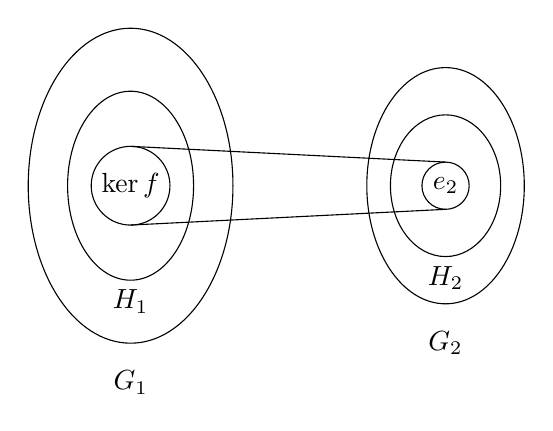
\begin{tikzpicture}
		\draw (-2,0) ellipse (1.3 and 2);
		\draw (2, 0) ellipse (1 and 1.5);
		\draw (-2,-2.5) node {$G_1$};
		\draw (2, -2) node {$G_2$};
		
		\node (ker) at (-2, 0) {$\ker f$};
		\node (e2) at (2,0) {$e_2$};
		
		\draw (ker) ellipse(.5 and .5);
		\draw (e2) ellipse (.3 and .3);
		\draw (-2,.5) -- (2,.3);
		\draw (-2,-.5) -- (2,-.3);
		
		% subgrupos de G1
		\draw (ker) ellipse (.8 and 1.2);
		\draw (-2,-1.2) node[anchor=north] {$H_1$};
		
		% subgrupos de G2
		\draw (e2) ellipse (.7 and .9);
		\draw (2, -.9) node[anchor=north] {$H_2$};
	\end{tikzpicture}
\end{figure}

\begin{ej}[Retículo de subgrupos de $\Z/8\Z$]
	Queremos saber sobre los subgrupos que tiene $\mathbb{Z}/8\mathbb{Z}$ (ver figura \ref{fig:reticulo8z}). El epimorfismo que utilizamos es $f:\Z \to \mathbb{Z}/8\mathbb{Z},\ z \mapsto f(z) = \overline{z}$ el habitual.
	
	Para ver los subgrupos de $\mathbb{Z}/8\mathbb{Z}$ miramos qué subgrupos de $\Z$ contienen a $\ker f = \{ z \in \Z \mid f(z) = \overline{0}\} = \{z \in \Z \mid z \mod 8 = 0\} = 8\Z$. Es decir, tenemos que encontrar los subgrupos de $\Z$ que contengan a los múltiplos de  8 ($8\Z$):
	\begin{align*}
	\Z \supset 2\Z \supset 4\Z \supset 8\Z
	\end{align*}
	En general, en $n\Z$, los subgrupos que contienen al núcleo son los $m\Z$ tales que $m \divides n$ ($m$ divide a $n$). 
	Luego $\mathbb{Z}/8\mathbb{Z}$ tendrá 4 subgrupos que serán $f(8\Z) = \mathbb{Z}/8\mathbb{Z}, f(4\Z) = \mathbb{Z}/4\mathbb{Z}, f(2\Z) = \mathbb{Z}/2\mathbb{Z}, f(\Z) = \{e\}$. 
\end{ej}

\begin{figure}[h]
	\centering
	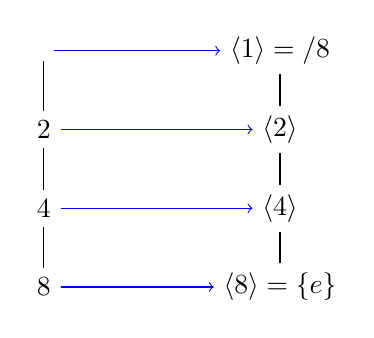
\begin{tikzpicture}
	% end nZ
	\node (z) at (-3,2) {$\Z$};
	\node (2z) at (-3,1) {$2\Z$};
	\node (4z) at (-3,0) {$4\Z$};
	\node (8z) at (-3,-1) {$8\Z$};
	
	\draw (8z) -- (4z);
	\draw (4z) -- (2z);
	\draw (2z) -- (z);
	
	% en Z/nZ
	\node (z8) at (0,2) {$\langle 1 \rangle = \Z/8\Z$};
	\node (z4) at (0,1) {$\langle 2 \rangle$};
	\node (z2) at (0,0) {$\langle 4 \rangle$};
	\node (e) at (0,-1) {$\langle 8 \rangle = \{e\}$};
	
	\draw (e) -- (z2);
	\draw (z2) -- (z4);
	\draw (z4) -- (z8);
	
	% las correspondencias
	\draw (z) edge[->, blue] (z8);
	\draw (2z) edge[->, blue] (z4);
	\draw (4z) edge[->, blue] (z2);
	\draw (8z) edge[->, blue] (e);
	\end{tikzpicture}
	
	\label{fig:reticulo8z}
	\caption{Retículo de subgrupos de $\mathbb{Z}/8\mathbb{Z}$}
\end{figure}

Lo mismo podríamos hacer para obtener el retículo de $\Z/6\Z$ (ver figura \ref{fig:reticulo6z}).

\begin{figure}[h]
	\centering
	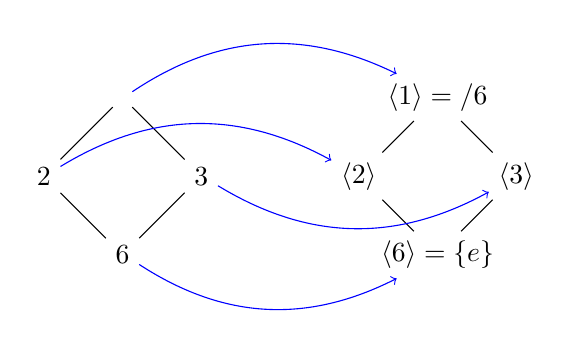
\begin{tikzpicture}
	% en nZ
	\node (z) at (-4, 1) {$\Z$};
	\node (2z) at (-5, 0) {$2\Z$};
	\node (3z) at (-3, 0) {$3\Z$};
	\node (6z) at (-4, -1) {$6\Z$};
	
	\draw (6z) -- (2z);
	\draw (6z) -- (3z);
	\draw (2z) -- (z);
	\draw (3z) -- (z);
	
	% en Z/nZ
	\node (z6) at (0,1) {$\langle 1 \rangle = \Z/6\Z$};
	\node (z2) at (-1,0) {$\langle 2 \rangle$};
	\node (z3) at (1,0) {$\langle 3\rangle$};
	\node (e) at (0,-1) {$\langle 6 \rangle = \{e\}$};
	
	\draw (e) -- (z2);
	\draw (e) -- (z3);
	\draw (z2) -- (z6);
	\draw (z3) -- (z6);
	
	% las correspondencias
	\draw (z) edge[->, bend left, blue] (z6);
	\draw (2z) edge[->, bend left, blue] (z2);
	\draw (3z) edge[->, bend right, blue] (z3);
	\draw (6z) edge[->, bend right, blue] (e);
	
	\end{tikzpicture}
	\label{fig:reticulo6z}
	\caption{Retículo de subgrupos de $\mathbb{Z}/6\mathbb{Z}$}
\end{figure}


\section{Teoremas de la isomorfía}

\begin{thm}(Primer teorema de la isomorfía)
	Sea $f:G_1 \to G_2$ un epimorfismo y sea $\pi:G_1 \to G_1/\ker f$. Entonces existe un isomorfismo $\overline{f} : G_1 / \ker f \to G_2$ tal que $f = \pi \circ \overline{f}$.
\end{thm}

\begin{figure}[h]
	%TODO hacer
	\centering
	\begin{tikzpicture}
	\node (g1) at (0,0) {$G_1$};
	\node (g2) at (4,0) {$G_2$};
	\node (gh) at (0, -3) {$G_1/\ker f$};
	
	\draw[-{Latex[length=2mm]}] (g1) -- (g2) node[pos=.5, above] {$f$};
	\draw[-{Latex[length=2mm]}] (g1) -- (gh) node[pos=.5, left]{$\pi$};
	\draw[-{Latex[length=2mm]}] (gh) -- (g2) node[pos=.5, below] {$\overline{f}$};
	\end{tikzpicture}
	\caption{Primer teorema de la isomorfía.}
	\label{fig:tmisomorfia1}
\end{figure}

\begin{thm}(Segundo teorema de la isomorfía)
	Sea $G$ un grupo, $H \normsub G,\ K \normsub G$ y $H < K$. Entonces $K/H$ es un subgrupo normal de $G/H$ y
	\begin{align}
		\sfrac{G/H}{K/H} \isom G/K
	\end{align}
\end{thm}

\begin{thm}[Tercer teorema de la isomorfía]
	Sea $G$ un grupo, $H < G,\ K \normsub G$. Entonces $HK < G$, $K \normsub HK$ y $H\cap K \normsub H$. Además,
	\begin{align}
		\sfrac{HK}{K} \isom \sfrac{H}{(H \cap K)}
	\end{align}
\end{thm}

Esta observación se utiliza para algunos problemas %TODO citar p.11 y p.14 de la hoja 1

\begin{obs}
	Sea $N \normsub G$ entonces $f:G \to G/N, f(x) = xN$ es un homomorfismo de grupos.
\end{obs}